\documentclass[a4paper,12pt]{article}
\usepackage[T2A]{fontenc}
\usepackage[utf8]{inputenc}
\usepackage[russian]{babel}
\usepackage{graphicx}
\usepackage{float}
\usepackage{amsmath}
\usepackage[margin=2.5cm]{geometry}
\graphicspath{{./}}
\begin{document}
\section*{Приложение. Графики и результаты}

\begin{figure}[H]\centering
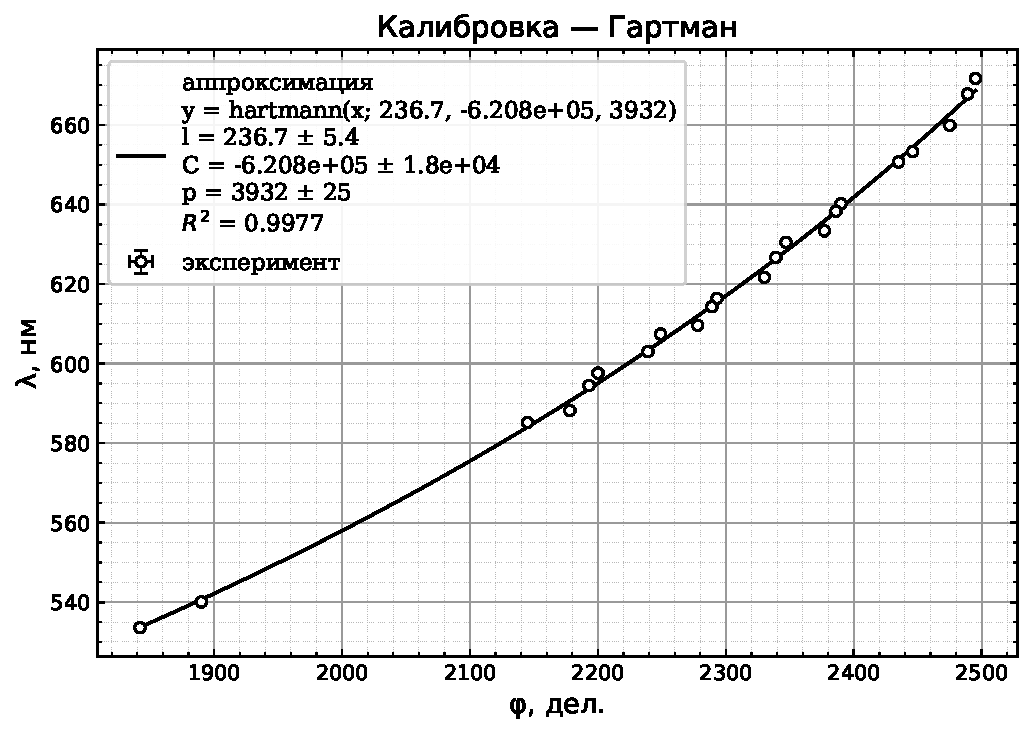
\includegraphics[width=0.82\textwidth]{fig_calib_hartmann.pdf}
\caption{Калибровочная кривая монохроматора, модель Гартмана.}
\end{figure}
\begin{center}\small
$\lambda_0=237\pm5.38$;\quad $C=-6.21\times10^{5}\pm1.82\times10^{4}$;\quad $\varphi_0=3932\pm24.6$;\quad $R^2=0.9977$.
\end{center}
\begin{figure}[H]\centering
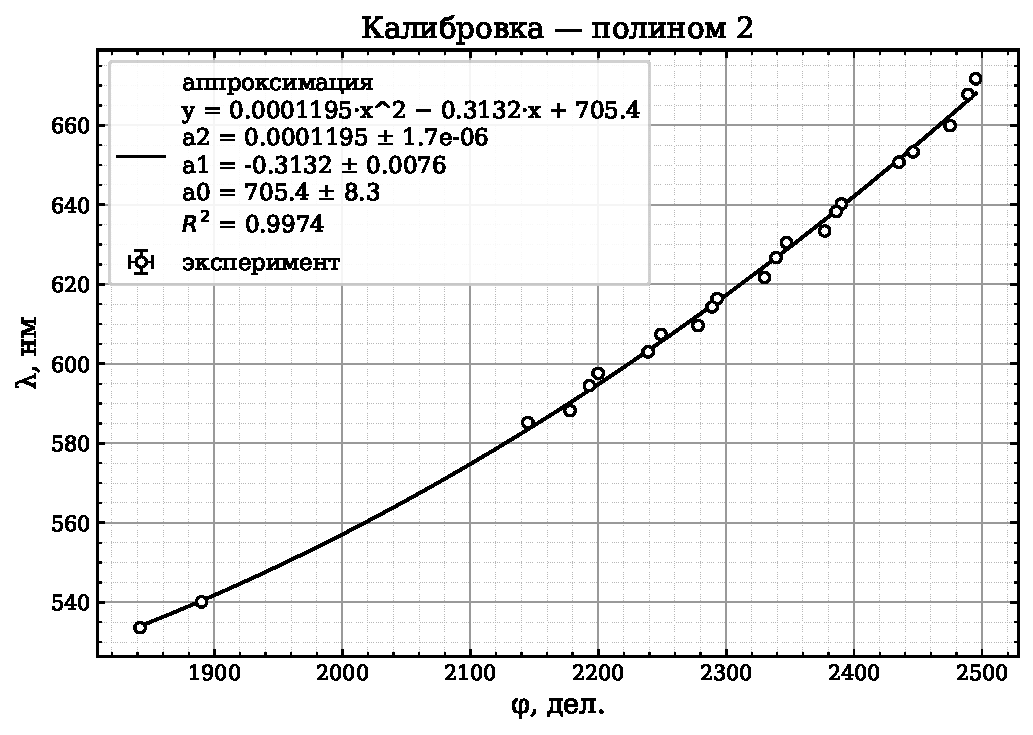
\includegraphics[width=0.82\textwidth]{fig_calib_poly.pdf}
\caption{Калибровочная кривая монохроматора, полином 2-й степени.}
\end{figure}
\begin{center}\small
$a_2=1.20\times10^{-4}\pm1.74\times10^{-6}$;\quad $a_1=-0.313\pm7.63\times10^{-3}$;\quad $a_0=705\pm8.31$;\quad $R^2=0.9974$.
\end{center}
\begin{figure}[H]\centering
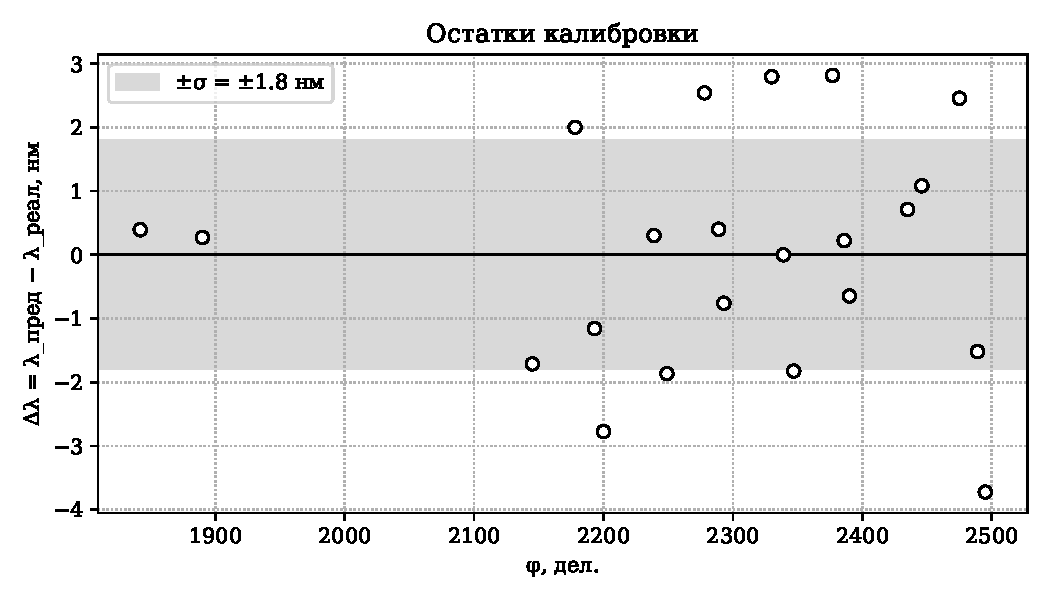
\includegraphics[width=0.82\textwidth]{fig_resid.pdf}
\caption{Остатки калибровки $\Delta\lambda=\lambda_\text{пред}-\lambda_\text{реал}$ (полином 2).}
\end{figure}
\begin{center}\small
RMS остатков $\sigma_\lambda=1.79$~нм.
\end{center}
\begin{figure}[H]\centering
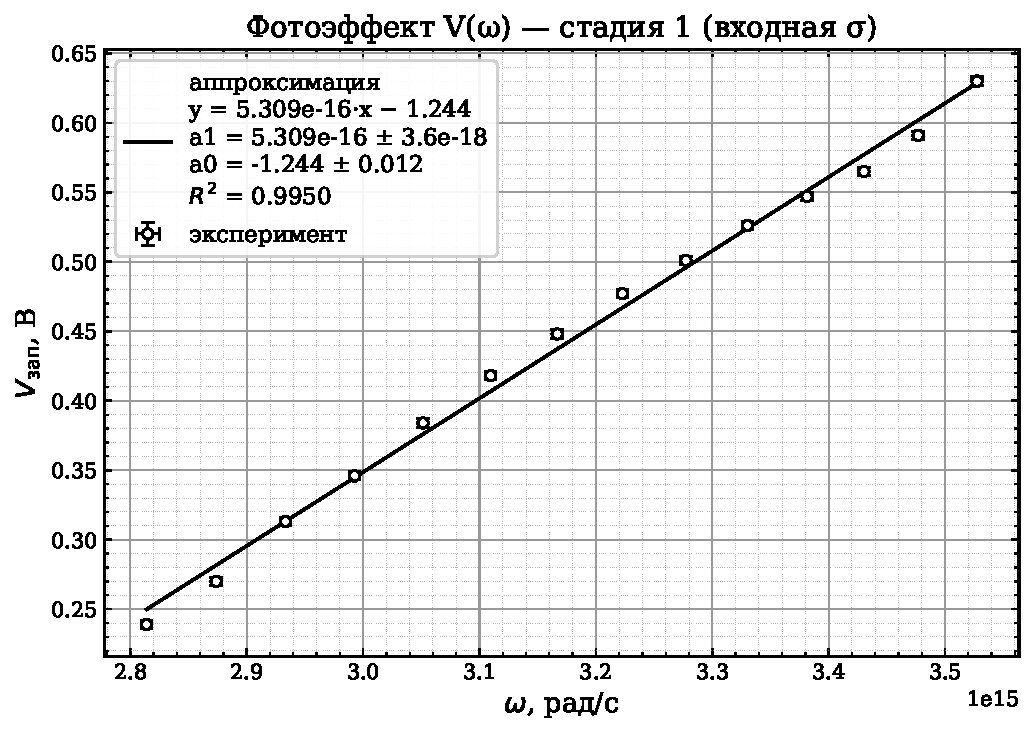
\includegraphics[width=0.82\textwidth]{fig_planck1.pdf}
\caption{Фотоэффект $V_\text{зап}(\omega)$, стадия 1 — входные погрешности.}
\end{figure}
\begin{center}\small
$\hbar=(8.51\times10^{-35}\pm5.78\times10^{-37})$~Дж$\cdot$с \ ($0.7\%$).
\end{center}
\begin{figure}[H]\centering
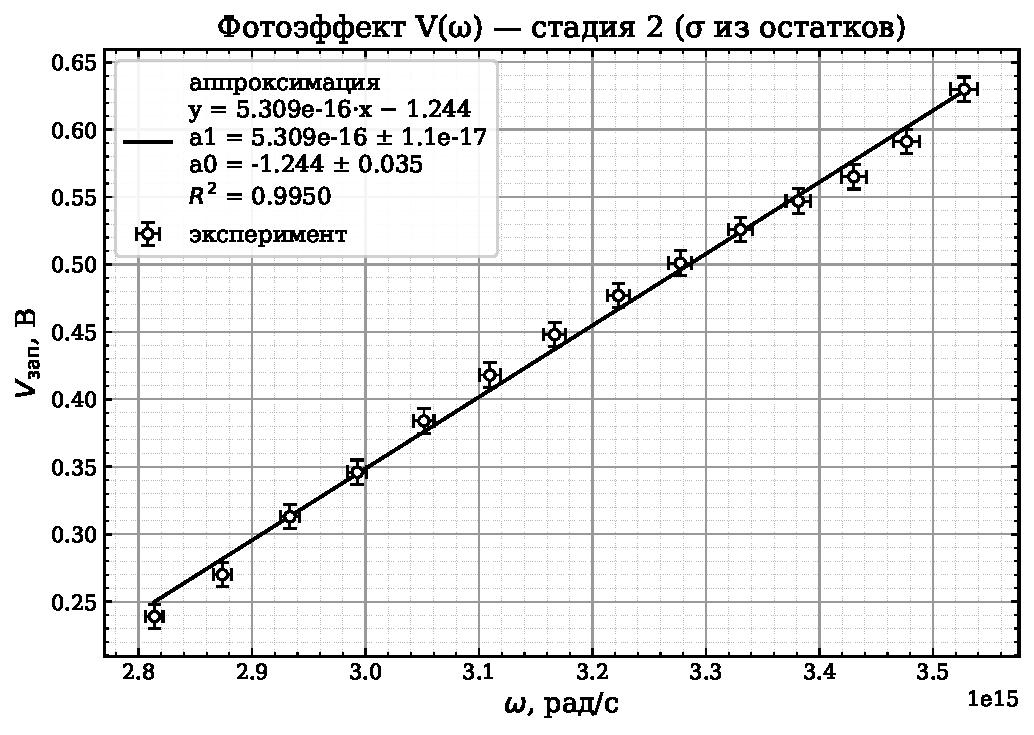
\includegraphics[width=0.82\textwidth]{fig_planck2.pdf}
\caption{Фотоэффект $V_\text{зап}(\omega)$, стадия 2 — погрешности из остатков (финал).}
\end{figure}
\begin{center}\small
$\sigma_V^\text{RMS}=0.0090$~В;\quad $\hbar=(8.51\times10^{-35}\pm1.74\times10^{-36})$~Дж$\cdot$с \ ($2.0\%$);\quad $\hbar_\text{табл}=1.05\times10^{-34}$~Дж$\cdot$с;\quad отклонение $-19\%$.
\end{center}

\end{document}
